% !TeX program = lualatex
% !TeX root = luaking.tex
% !TeX encoding = UTF-8
% !TeX spellcheck = cs_CZ
%---------------------------------------------------------------------------------------------------
% file fey1ch19.tex
%---------------------------------------------------------------------------------------------------
%=========================== Kapitola: Hmotný střed; Moment setrvačnosti ==========================
\setchaptertoc
\chapter{Hmotný střed; Moment setrvačnosti}\label{fyz:IchapXIX}
  \section{Vlastnosti hmotného středu}\label{fyz:IchapXIXsecI}
    V přecházející kapitole jsme zjistili, že, působí-li velmi mnoho sil na složitou soustavu
    částic, ať už jde o tuhé těleso, pružné těleso, hvězdný oblak nebo něco jiného, a sečteme-li
    všechny tyto síly (jsou to samozřejmě vnější síly, neboť vnitřní síly se vzájemně vyrušily) a
    díváme se na celý soubor částic jako na jedno těleso s celkovou hmotností \(M\), pak „uvnitř“
    existuje takový bod - hmotný střed (\emph{těžiště}) -, že výslednice vnějších sil působí taková
    zrychlení tohoto bodu, jakoby v něm byla soustředěna celá hmotnost souboru. Zabývejme se nyní
    hmotným středem trochu podrobněji.
    
    Poloha hmotného středu (ve zkratce \(T\)) je určena rovnicí
    \begin{equation}\label{fyz:eq739}
      \vec{R}_{CM}=\frac{∑m_ir_i}{∑m_i}.
    \end{equation}
    To je, jak je vidět, vektorová rovnice, která ve skutečnosti představuje tři rovnice (jednu pro
    každou ze tří souřadnic). Budeme se zabývat jen jednou, \(x\)-ovou souřadnicí, neboť
    porozumíme-li vztahům pro jednu souřadnicí, snadno je přeneseme na další dvě. Co znamená výraz
    \begin{equation}\label{fyz:eq740}
      X_{CM}=\frac{∑m_ix_i}{∑m_i}
    \end{equation}
    Předpokládejme, že těleso je rozděleno na malé části, z nichž každá má stejnou hmotnost \(m\).
    Celková hmotnost je pak rovna počtu částí \(N\) násobenému hmotností jednotlivé části. Tato
    rovnice pak znamená, že máme sčítat všechny polohy \(x_i\) a vydělit je počtem částí
    \begin{equation}\label{fyz:eq740}
      X_{CM} =  \frac{m∑x_i}{mN}= \frac{∑xi}{N}.
    \end{equation}
    
    \begin{figure}[ht!] %\ref{fyz:fig402}
      \centering
      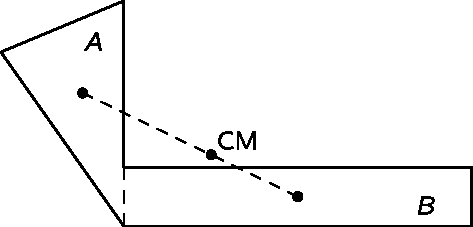
\includegraphics[width=0.8\linewidth]{fyz_fig402.pdf}
      \caption{Hmotný střed složeného tělesa leží na přímce spojující hmotné středy obou částí
              (\cite[s.~260]{Feynman01})}
      \label{fyz:fig402}
    \end{figure}

    Takže \(X_{CM}\) je střední hodnota všech \(x_i\) jsou-li všechny hmotnosti \(m_i\) stejné.
    Předpokládejme však, že některá část by byla dvakrát těžší než ostatní, pak by se příslušné
    \(x\) vyskytlo v součtu dvakrát To lze snadno pochopit, neboť tuto část s dvojnásobnou hmotností
    si můžeme představit rozdělenou na dvě poloviny, které jsou stejně těžké jako ostatní části. Při
    počítání průměru musíme příslušné \(x\) započítat dvakrát, neboť tam jsou takové části dvě.
    Takže \(X\) je průměrná poloha všech částí ve směru osy \(x\), přičemž poloha každé části se
    musí započítat úměrně ke své hmotnosti. Z toho lze snadno dokázat, že \(X\) musí ležet někde
    mezi největším a nejmenším \(x\), a proto leží uvnitř obalu ohraničujícího celé těleso. Nemusí
    se nacházet uvnitř materiálu samotného tělesa, neboť těleso může mít například tvar kružnice,
    jako prsten, kde hmotný střed je ve středu prstenu, a ne v samotném prstenu.

    Je-li těleso symetrické, například obdélník a má nějakou rovinu symetrie, pak hmotný střed leží
    někde v této rovině. V případě obdélníka existují dvě takové roviny, čímž je poloha hmotného
    středu určena jednoznačně. Jde-li o libovolné symetrické těleso, pak jeho hmotný střed leží
    někde na ose symetrie, neboť v takovém případě existuje stejný počet kladných i záporných \(x\).

    Všimněme si i dalšího zajímavého případu. Předpokládejme, že máme těleso složené ze dvou částí
    \(A\) a \(B\) (obr. \ref{fyz:fig402}). Hmotný střed celého tělesa pak lze vypočítat takovýmto
    způsobem: Nejdříve najdeme hmotný střed části \(A\), potom části \(B\) a zjistíme i hmotnost
    každé části \(M_A\) a \(M_B\). Pak budeme uvažovat nový problém, kdy hmota o hmotnosti \(M_A\)
    je soustředěna v bodě, jenž je hmotným středem \(A\), a hmota o hmotnosti \(M_B\) v bodě, jímž
    je hmotný střed tělesa \(B\). Hmotný střed těchto dvou hmotných bodů je pak hmotným středem
    celého tělesa. Jinak řečeno, jestliže jsme našli hmotný střed různých částí tělesa, nemusíme při
    výpočtu hmotného středu celého tělesa začínat úplně znova; stačí, když spojíme jednotlivé části,
    přičemž každou považujeme za hmotný bod umístěný v hmotném středu příslušné části. Podívejme se,
    proč je tomu tak. Předpokládejme, že chceme vypočítat hmotný střed celého tělesa, jehož dvě
    části patří k tělesu \(A\) a některé k tělesu \(B\). Celkovou sumu \(∑m_ix_i\) pak lze rozdělit
    na dvě části - sumu \(∑_Am_ix_i\) týkající se pouze tělesa \(A\) a sumu \(∑_Bm_ix_i\) vztahující
    se pouze k tělesu \(B\). Kdybychom počítali hmotný střed pouze tělesa \(A\), použili bychom
    první sumu, přičemž víme, že ta je rovna \(M_AX_A\) (celková hmotnost částí tělesa \(A\) krát
    poloha hmotného středu tělesa \(A\)) podle věty o hmotném středu aplikované na objekt \(A\).
    Rovněž pro těleso \(B\) máme \(M_BX_B\) a samozřejmě, že sečtením obou máme
    \begin{equation}\label{fyz:eq741}
      MX_{CM}=∑_Am_ix_i+∑_Bm_ix_i=M_AX_A+M_BX_B.
    \end{equation}

    Protože je jasné, že \(M\) je rovno součtu \(M_A\) a \(M_B\), vidíme, že rovnici
    (\ref{fyz:eq741}) lze interpretovat jako zvláštní případ vztahu pro výpočet hmotného středu dvou
    bodových těles, jednoho s hmotností \(M_A\) umístěného v bodě \(X_A\) a druhého s hmotností
    \(M_B\) v bodě \(X_B\).

    Věta o pohybu hmotného středu je velmi zajímavá a měla důležitou úlohu v rozvoji našeho chápání
    fyziky. Předpokládejme, že Newtonův zákon platí pro malé části mnohem většího tělesa. Pak podle
    této věty platí Newtonův zákon i pro větší těleso, ačkoli těleso neznáme detailně. Známe jen
    celkovou sílu, jež na něj působí a jeho hmotnost. Jinými slovy, Newtonův zákon má tu zvláštní
    vlastnost, že platí-li v určitém malém měřítku, bude platit i ve větším měřítku. Nebudeme-li
    míček považovat za velmi složitou věc skládající se z miliard interagujících částic a všimneme
    si pouze pohybu těžiště a vnějších sil působících na míček, zjistíme, že \(\vec{F}= m\vec{a}\),
    kde \(\vec{F}\) je vnější síla působící na míček, \(m\) je jeho hmotnost a \(\vec{a}\) je
    zrychlení jeho těžiště. Takže \(\vec{F}= m\vec{a}\) je zákon, který reprodukuje sám sebe ve
    větším měřítku. (Mělo by existovat slovo, možná řecké, k pojmenování zákona, který reprodukuje
    sám sebe ve větším měřítku.)

    Samozřejmě lze předpokládat, že zákony objevené jako první budou takové, jež se reprodukují ve
    větším měřítku. Proč? Protože měřítko základních „setrvačníků a koleček“ vesmíru má rozměry
    atomu, což je mnohem jemnější měřítko než nesrovnatelně větší měřítko našich běžných pozorování.
    Proto bychom jako první měli objevit zákony týkající se objektů, jejichž vlastnosti nejsou
    vázány na atomová měřítka. Kdyby se zákony platné pro malá tělesa nereprodukovaly ve větším
    měřítku, neobjevili bychom je tak snadno. Jak by to vypadalo, kdyby to bylo obráceně? Musí být
    zákony platné v malém měřítku stejné, jako zákony platné ve větším měřítku? V přírodě samozřejmě
    není nutné, aby zákony na úrovni atomových měřítek musely být stejné, jako zákony na úrovni
    větších měřítek. Předpokládejme, že by pravé zákony pohybu atomů byly dány nějakou podivnou
    rovnicí, která nemá vlastnost, že přejdeme-li k větším měřítkům, zreprodukuje se stejný zákon.
    Ale místo toho má tu vlastnost, že ve větších měřítkách ji lze aproximovat určitým výrazem,
    který když ho rozšíříme dál a dál, bude reprodukovat sám sebe ve větším a větším měřítku. To je
    možné a ve skutečnosti je tomu tak. Newtonovy zákony jsou „chvostem“ atomových zákonů
    extrapolovaných na velmi velké rozměry. Zákony pohybu částic v tom nejjemnějším měřítku jsou
    velmi zvláštní, ale když si vezmeme velké množství částic a složíme je, dostaneme přibližně ale
    jen přibližně, Newtonovy zákony. Newtonovy zákony nám pak umožňují, že můžeme přecházet k větším
    a větším měřítkům, přičemž se zdá, že platí stále stejný zákon. Ve skutečnosti dokonce, jak se
    měřítko zvětšuje, stává se zákon stále přesnějším a přesnějším. Samoreprodukční faktor
    Newtonových rovnic není sice základní vlastností přírody, je však důležitý po historické
    stránce. Základní zákony atomových částic bychom nikdy neobjevili při prvním pozorování, neboť
    první pozorování jsou příliš hrubá. Opravdu se ukazuje, že základní atomové zákony, jež nazýváme
    kvantovou mechanikou, se zcela liší od Newtonových zákonů. Lze je těžko pochopit, neboť všechny
    naše přímé zkušenosti máme s objekty velkých měřítek a chování atomů je zcela jiné než to, co
    vidíme ve velkých měřítkách. Proto nemůžeme říct: „Elektron v atomu je jako planeta obíhající
    kolem Slunce“ nebo něco podobného. Není to jako nic, co známe, protože nic se mu nepodobá. Když
    aplikujeme kvantovou mechaniku na stále větší a větší tělesa, zákony chování mnoha atomů se
    nezreprodukují, ale dostaneme z nich nové zákony - Newtonovy zákony. Ty se potom reprodukují
    počínaje řekněme měřítkem milióntiny mikrogramu, což již představuje miliardy a miliardy atomů,
    až k rozměrům Země a dále. 
    
    Nyní se vraťme k hmotnému středu. Často se nazývá i těžištěm, a to proto, že ve většině případů
    je gravitační pole stejnorodé. Předpokládejme, že máme dostatečně malé rozměry, takže gravitační
    síla není jen úměrná hmotnosti, ale všude je i rovnoběžná s daným směrem. Mějme těleso, na jehož
    všechny části hmoty působí gravitační síly. Nechť mí je hmotnost jedné části. Gravitační síla
    působící na tuto část je pak \(m_i\) krát \(g\). Zůstává otázkou, v kterém bodě máme působit
    jedinou silou tak, abychom vyvážili gravitační sílu působící na těleso a aby se celý objekt
    (jde-li o tuhé těleso) neotáčel? Odpověď je, že síla musí procházet hmotným středem. Dokážeme
    to: Aby se těleso neotáčelo, musí se součet momentů všech sil rovnat nule, neboť kde je moment
    síly, tam je i změna momentu hybnosti, tedy rotace. Proto musíme spočítat momenty sil působící
    na všechny částice a zjistit, jak velký je výsledný moment síly vzhledem k nějaké ose (když osa
    prochází hmotným středem, měl by být nulový). Když budeme \(x\) měřit horizontálně a \(y\)
    vertikálně, budou momenty sil rovny velikostem sil ve směru \(y\), jež vynásobíme velikostí
    příslušného ramene ve směru \(x\) (podle pravidla síla krát rameno síly vzhledem k ose, vůči níž
    určujeme moment síly). Celkový moment síly je roven součtu
    \begin{equation}\label{fyz:eq742}
      τ=∑m_igx_i=g∑m_ix_i,
    \end{equation}
    Proto má-li být celkový moment síly roven nule, musí být součet \(∑m_ix_i\) roven nule. Ale
    \(∑m_ix_i=MX_{CM}\), tj. celková hmotnost krát vzdálenost hmotného středu od osy otáčení, proto
    \(x\)-ová vzdálenost hmotného středu od osy otáčení je rovna nule.



  \section{Poloha hmotného bodu}\label{fyz:IchapXIXsecII}
  \section{Určení momentu setrvačnosti}\label{fyz:IchapXIXsecIII}
  \section{Kinetická energie rotace}\label{fyz:IchapXIXsecIV}
  \section{Příklady a cvičení}\label{fyz:IchapXIXsecV}



    \begin{figure}[ht!] %\ref{fyz:fig403}
      \centering
      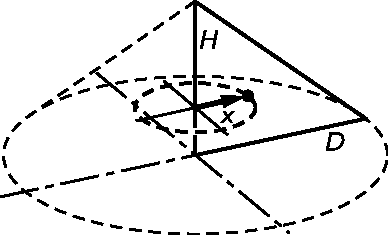
\includegraphics[width=0.3\linewidth]{fyz_fig403.pdf}
      \caption{Pravoúhlý trojúhelník a přímý rotační kužel vytvořený rotujícím trojúhelníkem 
              (\cite[s.~263]{Feynman01})}
      \label{fyz:fig403}
    \end{figure}
    \begin{figure}[ht!] %\ref{fyz:fig404}
      \centering
      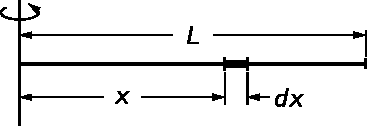
\includegraphics[width=0.3\linewidth]{fyz_fig404.pdf}
      \caption{Přímá tyč \(L\) rotující kolem osy procházející jedním koncem
              (\cite[s.~264]{Feynman01})}
      \label{fyz:fig404}
    \end{figure}

    \begin{figure}[ht!] %\ref{fyz:fig405}
      \centering
      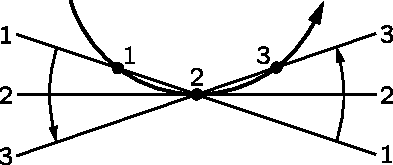
\includegraphics[width=0.3\linewidth]{fyz_fig405.pdf}
      \caption{Tři postupné pohledy na radiálně se pohybující bod na otáčející se podložce
              (\cite[s.~269]{Feynman01})}
      \label{fyz:fig405}
    \end{figure}
%---------------------------------------------------------------------------------------------------